\section{Implementation}

\let\plaintextsf=\textsf
\def\textsf#1{\plaintextsf{\small #1}}

\subsection{Data Model Language}

The data model language was implemented using the Eclipse Modeling
Framework (EMF)~\cite{EMF}, with the class and association entities
being based upon Ecore~\cite{ECORE} classes.  Additional metaclasses
were included to represent attributes as \emph{data elements}, and the
range of values permitted as \emph{value domains}.  A value domain has
an associated \emph{datatype}, specifying representation, with an
optional notion of \emph{units}.

Language extensions for specific implementation types were implemented
in the same framework.  As an example, consider the metamodel for
forms shown in Figure~\ref{fig:formsmodel}, which includes an
additional class \textsf{Section} alongside the core classes
\textsf{DataClass}, \textsf{DataElement}, \textsf{DataConstraint}, and
\textsf{DataAssociation}.  This class may \textsf{contain} any
\textsf{DataConcept}, including \textsf{Section} itself.  As a
subclass of \textsf{DataConcept}, it can be linked to data concepts in
other models.  Other metaclasses, including \textsf{ValueDomain} are
not shown.

\begin{figure}[h]
  \centering
  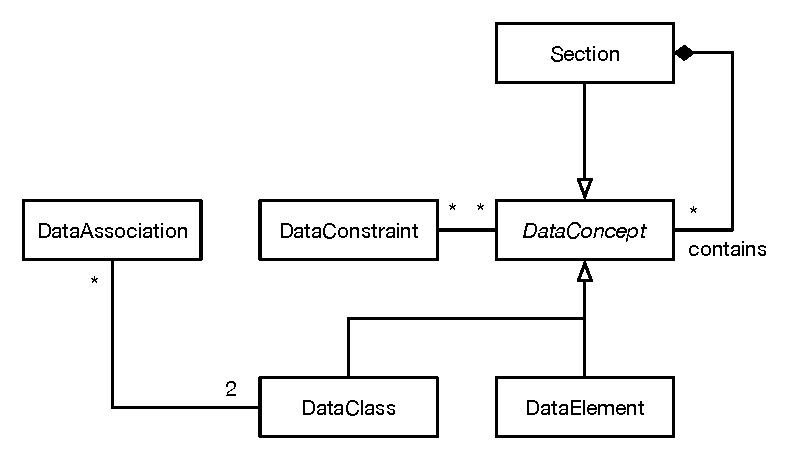
\includegraphics[width=\columnwidth]{ASEFigs/languageExtensionExample}
  \caption{Extending the data model language}
  \label{fig:formsmodel}
\end{figure}

\subsection{Model Catalogue}

The model catalogue stores classes, data elements, constraints, and
associations only as components of data models.  It stores also
administrative links between models---recording, for example, the fact
that one model is a new version of another---and semantic links
between data concepts: classes and elements.  

In the current version of the catalogue, associations are not
considered as concepts for semantic linking.  The instantiation of an
association as a reference type is a platform-specific concern, and
thus associations are quite different from ordinary data elements or
attributes, in having only an abstract notion of a value domain.  

At present, if we wish to reason about an association as a concept, we
need to introduce an explicit reference or identifier type into our
model.  This is analogous to the use of foreign keys in a relational
database.  It would, however, be a relatively straightforward matter
to allow linking of associations as abstract data concepts. 

\begin{figure}[h]
  \centering
  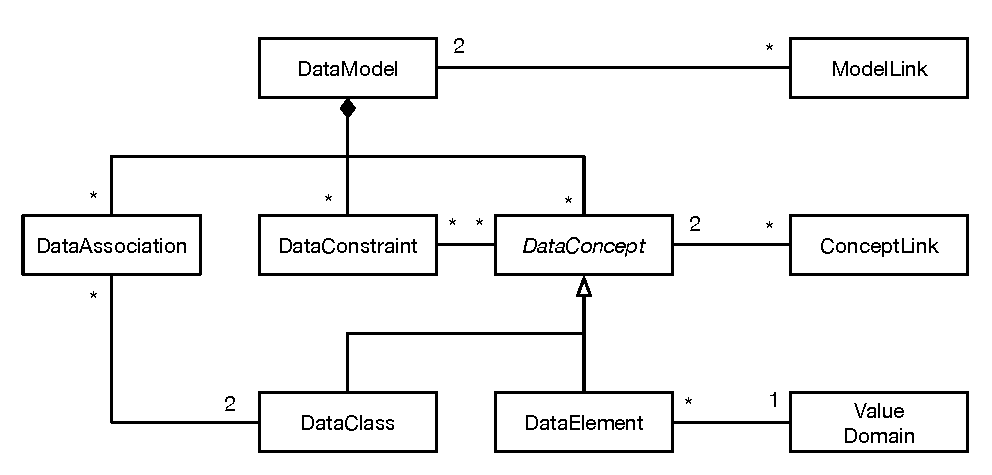
\includegraphics[width=\columnwidth]{ASEFigs/modelCatalogueContents}
  \caption{Model catalogue contents}
  \label{fig:catalogueContents}
\end{figure}

Figure~\ref{fig:catalogueContents} is a simplified representation of
the information stored.  The actual implementation includes also the
notion of a \textsf{ValueConcept}, which may be used to support
semantic linking of value domains and---in the case of an enumerated
value domain---the value elements they contain.

\subsection{Metadata registration}

In designing the language, we gave due consideration to the ISO/IEC
11179 international standard for metadata registration.  This standard
sets out a metamodel for data definitions, together with a set of
processes for their registration and publication: the core set of
metaclasses is shown in Figure~\ref{fig:11179}. 

\begin{figure}[h]
  \centering
  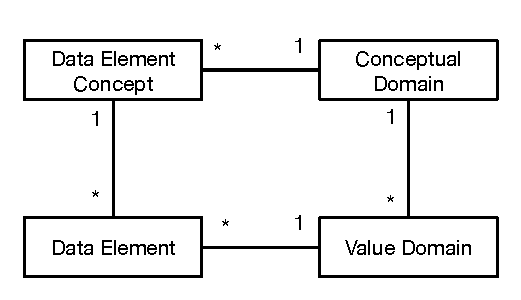
\includegraphics[width=0.75\columnwidth]{ASEFigs/11179metamodel}
  \caption{ISO/IEC 11179 core metaclasses} 
  \label{fig:11179}
\end{figure}

In the ISO/IEC 11179 standard, data elements correspond to individual
data points and may be grouped or classified into `data element
concepts'.  Each concept represents a set of data elements that are
capturing `conceptually' the same information: for example, different
ways of measuring blood pressure.  Value domains are classified into
`conceptual domains', representing different ways of recording the
same kind of observations. 

The only other form of semantic link supported by the standard is the
classification of data element concepts according a single
property-based hierarchy.  A single classification scheme is unlikely
to capture semantic information in a way that suits the purposes of
different users, and represents a problem for registration: who is to
decide quite where a new data element fits within the existing
hierarchy?  

The approach taken in our implementation of the model catalogue is
more general: the use of semantic links supports multiple
classification schemes, and allows the representation of relationships
other than simple taxonomies.  However, it should be clear that our
catalogue could be used, under suitable constraints, as an effective
implementation of the ISO/IEC 11179 standard. 

This applies also to the processes of registration, versioning, and
publication.  Every object stored in the catalogue is managed as an
\emph{administered item}, in the language of the standard.  The richer
notion of linking in the catalogue implementation allows us to exploit
this administrative information in the automatic creation and
maintenance of semantic links, and the administrative processes are
generalised to provide support for collaborative development, but the
option of a constrained form of implementation remains. 

\subsection{Technology platform}

The existing model catalogue is built using the Groovy/Grails
framework, which takes a model-view-controller approach to data
management and presentation.  The key advantage of this platform has
been the ability to revisit the underlying data representation---the
domain model---without needing to re-implement the presentation
layer, and vice versa.  As the software was developed in the course of
application, this was particularly important. 

The plug-in architecture of the framework allowed us to add in
cross-cutting features---such as global search, access control, and a
collaboration environment---without re-engineering the data
representation and presentation aspects.  This architecture, and the
built-in support for domain-specific langauges, was particularly
helpful in the development of model import and export pipelines: 
facilitating the generation and configuration of software artefacts
from models, as well as the generation of models for existing
artefacts.

The web interface was developed using the AngularJS JavaScript
library, which worked well in support of the continuing interation of
the design through interaction and collaboration with users.  Although
the users were highly-skilled clinical scientists, they had little or
no intuition or experience in data modelling.  Concepts such as
inheritance, reference, composition, and instantiation were unfamiliar
and confusing to them.  Only through close collaboration were we able
to develop a presentation of these concepts that they found
accessible.

The persistence layer was implemented using the Grails Object
Relational Mapping (GORM), enhancing portability but creating some
concerns with regard to scalability: no performance issues have been
encountered to date, but the potential exponential increase in
complexity, as further linked models are added, and further
relationships are inferred, means that an alternative platform may
need to be considered. 

\begin{figure}[here]
  \centering
  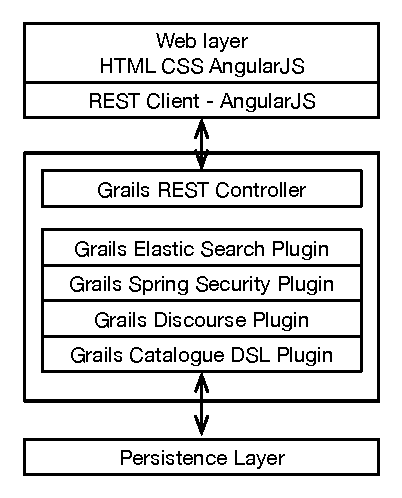
\includegraphics[width=0.5\columnwidth]{architecture}
  \caption{Implementation architecture}
  \label{fig:architecture}
\end{figure}

The current technology stack is shown in
Figure~\ref{fig:architecture}.  The discourse plugin provides support
for collaborative development of models and data definitions, with
users able to contribute to a comment history for each administered
item, prompting responses from other users as necessary.  This proved
particularly important given that many of the clinical scientists were
contributing to the dataset development in their spare time. 

\subsection{Generation pipelines}

The existing implementation has been used to generate several
different types of artefact, including:

\paragraph{Case report form models for consumption by the OpenClinica
  clinical trials management system}  These take the form of Excel
spreadsheets with columns specifying form structure, question text,
response types, logical constraints (including skip logic), and
presentation controls.  These models are generated from form models in
the data modelling language by way of a complex transformation: the
hierarchical structure of the data model is flattened to produce lists
of sections, repeating groups, and questions.  Default values and
implementations are included as part of the transformation: for
example, we provide custom validation for textual fields that are
tagged with constraints in the form of regular expressions.

\paragraph{Database triggers} To support the automatic processing of
data received from the clinical trials system, we require a collection
of triggers for the underlying database.  These ensure that the
combination of existing and newly-received data is properly
normalised.  This is particularly important where data is being
collected against different versions of the same form.

\paragraph{XML schemas for electronic document submission}  This is a
more straightforward transformation, as the structure of the XML
schemas is closer to that of the data models.  However, additional
processing is required to produce normalised, readable schemas.  For
example, if there are several data elements sharing the same value
domain, we would wish to include that value domain only once within
the schema.

\paragraph{Tools for creating and validating .csv files}  For some of
the systems that we are working with, the easiest way to import or
export information is in comma-separated value format.  In this case,
we are not generating a specification of the data format in some
implementation language; we are instead generating tools that will
ensure that the values presented in a file comply with the model
constraints.

\paragraph{Data manuals}  Datasets and data standards in health
  informatics are communicated through documents in which each data
  point is listed along with its intended interpretation.  By
  generating these manuals automatically, we are able to ensure
  consistency between the information that they present and the tools
  used for data acquisition and processing.  The models used to
  generate the manual are semantically linked to those used for XML
  schema and case report form generation. 

